%\documentclass[handout]{beamer}
\documentclass{beamer}
%\usepackage{beamerthemesplit}
%\usepackage{logicthemelive}
\usepackage{cite}
\usepackage{enumitem}
\usepackage{pgf}
\usepackage{tikz}
\usepackage{graphicx}
\usepackage{datatool}
\usepackage{dataplot}
\usepackage{xcolor}
\usetikzlibrary{calc,through,decorations.pathmorphing}
\usetikzlibrary{decorations.text}
\usetikzlibrary{trees}
\usetikzlibrary{fit}
\usetikzlibrary{backgrounds}
\usetikzlibrary{positioning}
\usetikzlibrary{shapes,arrows}
\usetikzlibrary{shadows}
\usetikzlibrary{calendar}
%\usepackage[cmex10]{amsmath}
%\usepackage{array}
\usepackage{ctable}
\usepackage{dcolumn}
\usepackage{mdwmath}
\usepackage{mdwtab}
\usepackage{setspace}
\usepackage{fancyhdr}
%\usepackage{electComp}
%\usepackage{amsmath}

\title[Options for improved loss modelling in the New Zealand Electricity Market]{\Large Options for improved loss modelling in the New Zealand Electricity Market}
%\author{Dr David Hume}
%\subtitle{\tiny EEA Conference - 23rd June, 2011} % (optional)
%\author[David Hume]{\normalsize David Hume \\ \tiny {\texttt{david.hume@ea.govt.nz}} \\ \tiny Electricity Authority of New Zealand}
%\institute{\tiny Electricity Authority of New Zealand}
\date{}



\begin{document}

\frame{\titlepage}


%\frame{\tableofcontents}

\section[Effect of power factor on power transfer -- thermal limits]{Effect of power factor on power transfer -- thermal limits}

 
\frame{
 \frametitle{Loss segment approximation -- 2 segments}
\vspace{-10mm}
\begin{center}
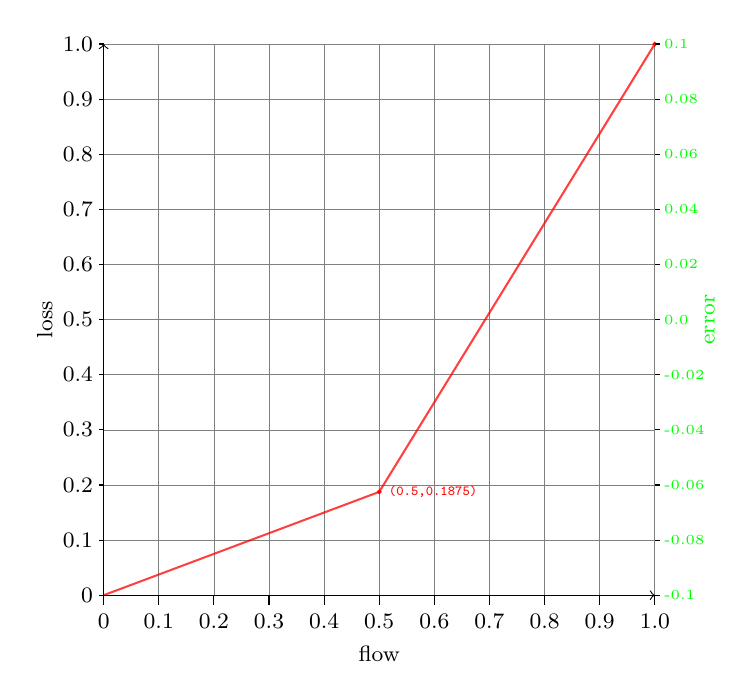
\begin{tikzpicture}[xscale=7.0,yscale=7.0]
\draw [help lines,step=0.1] (0,0) grid (1,1);
\draw[line width=0.5pt,color=black] plot file {default_2_XY.dat};
\coordinate (oneone) at (1,1);
\filldraw [red,draw opacity=0.75] (oneone) circle (0.1pt);
\coordinate (bk1) at (0,0);
\coordinate (bk2) at (0.5,0.1875);
\coordinate (bk3) at (1,1);
\filldraw [red,draw opacity=0.75] (bk2) circle (0.1pt) node[right] {\tiny \texttt{(0.5,0.1875)}};
\draw[line width=0.75pt,color=red,draw opacity=0.75] (bk1) -- (bk2); 
\draw[line width=0.75pt,color=red,draw opacity=0.75] (bk2) -- (bk3); 
\draw[->] (0,0) -- node[midway,yshift=-0.75cm] {\footnotesize flow} (1,0);
\draw[->] (0,0) -- node[rotate=90,midway,yshift=0.75cm] {\footnotesize loss} (0,1) ;
\foreach \x/\xtext in {0,0.1,0.2,0.3,0.4,0.5,0.6,0.7,0.8,0.9,1.0}
\draw (\x cm,0pt) -- (\x cm,-0.5pt) node[anchor=north] {\footnotesize \xtext};
\foreach \y/\ytext in {0,0.1,0.2,0.3,0.4,0.5,0.6,0.7,0.8,0.9,1.0}
\draw (0.0pt,\y cm) -- (-0.25pt,\y cm) node[anchor=east,xshift=0.5mm] {\footnotesize \ytext};
\draw[line width=0.5pt,color=green,draw opacity=0.75] plot file {default_2_err.dat};
\foreach \y/\ytext in {0/-0.1,0.1/-0.08,0.2/-0.06,0.3/-0.04,0.4/-0.02,0.5/0.0,0.6/0.02,0.7/0.04,0.8/0.06,0.9/0.08,1.0/0.1}
\draw (1cm,\y cm) -- (1.01cm,\y cm) node[anchor=west,xshift=-0.75mm] {\tiny \textcolor{green}{\ytext}};
\node[rotate=90] at (1.1,0.5) {\footnotesize \textcolor{green}{error}};
\end{tikzpicture}

\end{center}
}

\frame{
 \frametitle{Loss segment approximation -- 3 segments}
\vspace{-10mm}
\begin{center}
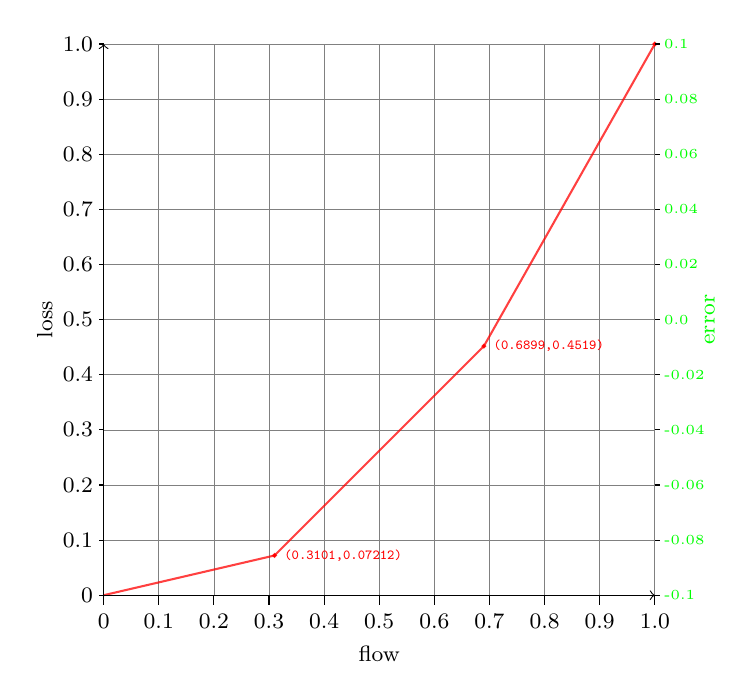
\begin{tikzpicture}[xscale=7.0,yscale=7.0]
\draw [help lines,step=0.1] (0,0) grid (1,1);
\draw[line width=0.5pt,color=black] plot file {default_3_XY.dat};
\coordinate (oneone) at (1,1);
\filldraw [red,draw opacity=0.75] (oneone) circle (0.1pt);
\coordinate (bk1) at (0,0);
\coordinate (bk2) at (0.31009,0.072116);
\coordinate (bk3) at (0.68989,0.45191);
\coordinate (bk4) at (1,1);
\filldraw [red,draw opacity=0.75] (bk2) circle (0.1pt) node[right] {\tiny \texttt{(0.3101,0.07212)}};
\filldraw [red,draw opacity=0.75] (bk3) circle (0.1pt) node[right] {\tiny \texttt{(0.6899,0.4519)}};
\draw[line width=0.75pt,color=red,draw opacity=0.75] (bk1) -- (bk2); 
\draw[line width=0.75pt,color=red,draw opacity=0.75] (bk2) -- (bk3); 
\draw[line width=0.75pt,color=red,draw opacity=0.75] (bk3) -- (bk4); 
\draw[->] (0,0) -- node[midway,yshift=-0.75cm] {\footnotesize flow} (1,0);
\draw[->] (0,0) -- node[rotate=90,midway,yshift=0.75cm] {\footnotesize loss} (0,1) ;
\foreach \x/\xtext in {0,0.1,0.2,0.3,0.4,0.5,0.6,0.7,0.8,0.9,1.0}
\draw (\x cm,0pt) -- (\x cm,-0.5pt) node[anchor=north] {\footnotesize \xtext};
\foreach \y/\ytext in {0,0.1,0.2,0.3,0.4,0.5,0.6,0.7,0.8,0.9,1.0}
\draw (0.0pt,\y cm) -- (-0.25pt,\y cm) node[anchor=east,xshift=0.5mm] {\footnotesize \ytext};
\draw[line width=0.5pt,color=green,draw opacity=0.75] plot file {default_3_err.dat};
\foreach \y/\ytext in {0/-0.1,0.1/-0.08,0.2/-0.06,0.3/-0.04,0.4/-0.02,0.5/0.0,0.6/0.02,0.7/0.04,0.8/0.06,0.9/0.08,1.0/0.1}
\draw (1cm,\y cm) -- (1.01cm,\y cm) node[anchor=west,xshift=-0.75mm] {\tiny \textcolor{green}{\ytext}};
\node[rotate=90] at (1.1,0.5) {\footnotesize \textcolor{green}{error}};
\end{tikzpicture}

\end{center}
}

\frame{
 \frametitle{Loss segment approximation -- 4 segments}
\vspace{-10mm}
\begin{center}
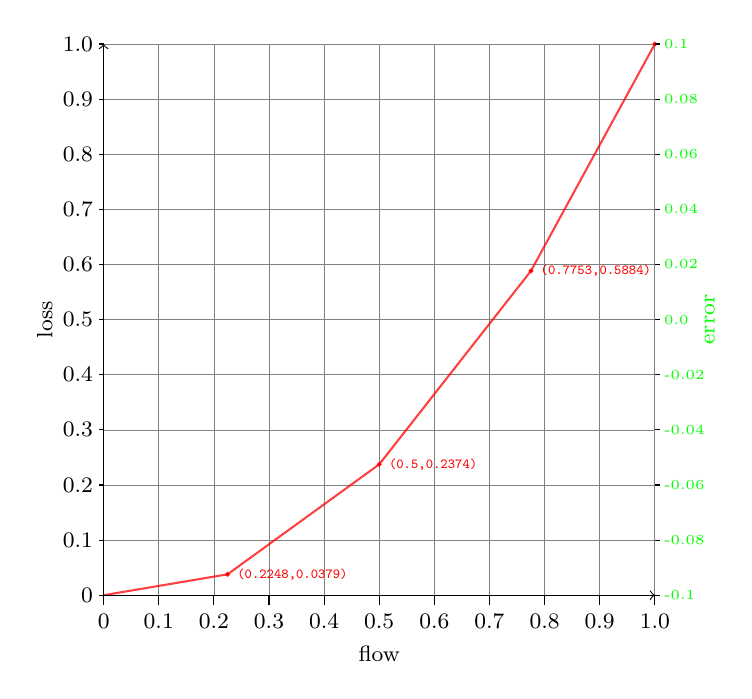
\begin{tikzpicture}[xscale=7.0,yscale=7.0]
\draw [help lines,step=0.1] (0,0) grid (1,1);
\draw[line width=0.5pt,color=black] plot file {default_4_XY.dat};
\coordinate (oneone) at (1,1);
\filldraw [red,draw opacity=0.75] (oneone) circle (0.1pt);
\coordinate (bk1) at (0,0);
\coordinate (bk2) at (0.22479,0.037898);
\coordinate (bk3) at (0.50005,0.23742);
\coordinate (bk4) at (0.77528,0.58843);
\coordinate (bk5) at (1,1);
\filldraw [red,draw opacity=0.75] (bk2) circle (0.1pt) node[right] {\tiny \texttt{(0.2248,0.0379)}};
\filldraw [red,draw opacity=0.75] (bk3) circle (0.1pt) node[right] {\tiny \texttt{(0.5,0.2374)}};
\filldraw [red,draw opacity=0.75] (bk4) circle (0.1pt) node[right] {\tiny \texttt{(0.7753,0.5884)}};
\draw[line width=0.75pt,color=red,draw opacity=0.75] (bk1) -- (bk2); 
\draw[line width=0.75pt,color=red,draw opacity=0.75] (bk2) -- (bk3); 
\draw[line width=0.75pt,color=red,draw opacity=0.75] (bk3) -- (bk4); 
\draw[line width=0.75pt,color=red,draw opacity=0.75] (bk4) -- (bk5); 
\draw[->] (0,0) -- node[midway,yshift=-0.75cm] {\footnotesize flow} (1,0);
\draw[->] (0,0) -- node[rotate=90,midway,yshift=0.75cm] {\footnotesize loss} (0,1) ;
\foreach \x/\xtext in {0,0.1,0.2,0.3,0.4,0.5,0.6,0.7,0.8,0.9,1.0}
\draw (\x cm,0pt) -- (\x cm,-0.5pt) node[anchor=north] {\footnotesize \xtext};
\foreach \y/\ytext in {0,0.1,0.2,0.3,0.4,0.5,0.6,0.7,0.8,0.9,1.0}
\draw (0.0pt,\y cm) -- (-0.25pt,\y cm) node[anchor=east,xshift=0.5mm] {\footnotesize \ytext};
\draw[line width=0.5pt,color=green,draw opacity=0.75] plot file {default_4_err.dat};
\foreach \y/\ytext in {0/-0.1,0.1/-0.08,0.2/-0.06,0.3/-0.04,0.4/-0.02,0.5/0.0,0.6/0.02,0.7/0.04,0.8/0.06,0.9/0.08,1.0/0.1}
\draw (1cm,\y cm) -- (1.01cm,\y cm) node[anchor=west,xshift=-0.75mm] {\tiny \textcolor{green}{\ytext}};
\node[rotate=90] at (1.1,0.5) {\footnotesize \textcolor{green}{error}};
\end{tikzpicture}

\end{center}
}

\frame{
 \frametitle{Loss segment approximation - 5 segments}
\vspace{-10mm}
\begin{center}
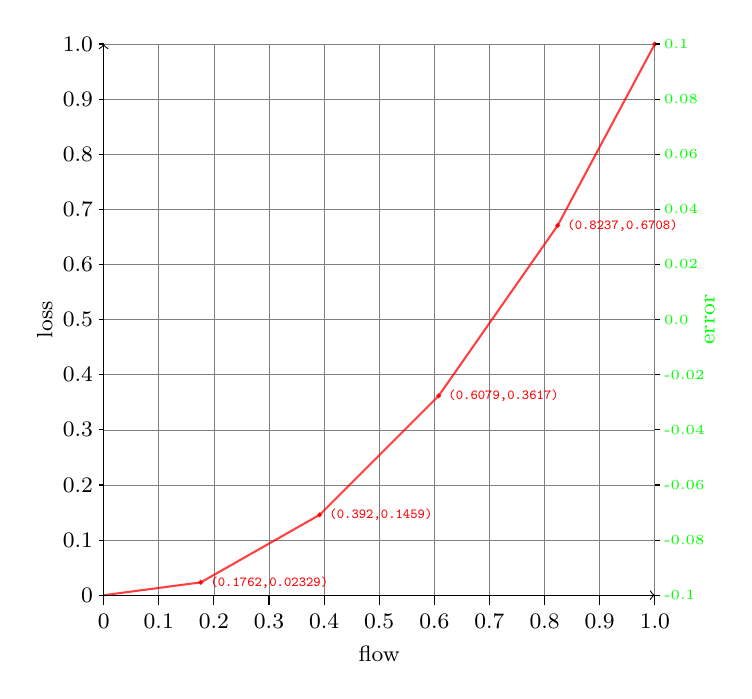
\begin{tikzpicture}[xscale=7.0,yscale=7.0]
\draw [help lines,step=0.1] (0,0) grid (1,1);
\draw[line width=0.5pt,color=black] plot file {default_5_XY.dat};
\coordinate (oneone) at (1,1);
\filldraw [red,draw opacity=0.75] (oneone) circle (0.1pt);
\coordinate (bk1) at (0,0);
\coordinate (bk2) at (0.17621,0.023287);
\coordinate (bk3) at (0.39202,0.14592);
\coordinate (bk4) at (0.60787,0.36174);
\coordinate (bk5) at (0.82374,0.67078);
\coordinate (bk6) at (1,1);
\filldraw [red,draw opacity=0.75] (bk2) circle (0.1pt) node[right] {\tiny \texttt{(0.1762,0.02329)}};
\filldraw [red,draw opacity=0.75] (bk3) circle (0.1pt) node[right] {\tiny \texttt{(0.392,0.1459)}};
\filldraw [red,draw opacity=0.75] (bk4) circle (0.1pt) node[right] {\tiny \texttt{(0.6079,0.3617)}};
\filldraw [red,draw opacity=0.75] (bk5) circle (0.1pt) node[right] {\tiny \texttt{(0.8237,0.6708)}};
\draw[line width=0.75pt,color=red,draw opacity=0.75] (bk1) -- (bk2); 
\draw[line width=0.75pt,color=red,draw opacity=0.75] (bk2) -- (bk3); 
\draw[line width=0.75pt,color=red,draw opacity=0.75] (bk3) -- (bk4); 
\draw[line width=0.75pt,color=red,draw opacity=0.75] (bk4) -- (bk5); 
\draw[line width=0.75pt,color=red,draw opacity=0.75] (bk5) -- (bk6); 
\draw[->] (0,0) -- node[midway,yshift=-0.75cm] {\footnotesize flow} (1,0);
\draw[->] (0,0) -- node[rotate=90,midway,yshift=0.75cm] {\footnotesize loss} (0,1) ;
\foreach \x/\xtext in {0,0.1,0.2,0.3,0.4,0.5,0.6,0.7,0.8,0.9,1.0}
\draw (\x cm,0pt) -- (\x cm,-0.5pt) node[anchor=north] {\footnotesize \xtext};
\foreach \y/\ytext in {0,0.1,0.2,0.3,0.4,0.5,0.6,0.7,0.8,0.9,1.0}
\draw (0.0pt,\y cm) -- (-0.25pt,\y cm) node[anchor=east,xshift=0.5mm] {\footnotesize \ytext};
\draw[line width=0.5pt,color=green,draw opacity=0.75] plot file {default_5_err.dat};
\foreach \y/\ytext in {0/-0.1,0.1/-0.08,0.2/-0.06,0.3/-0.04,0.4/-0.02,0.5/0.0,0.6/0.02,0.7/0.04,0.8/0.06,0.9/0.08,1.0/0.1}
\draw (1cm,\y cm) -- (1.01cm,\y cm) node[anchor=west,xshift=-0.75mm] {\tiny \textcolor{green}{\ytext}};
\node[rotate=90] at (1.1,0.5) {\footnotesize \textcolor{green}{error}};
\end{tikzpicture}

\end{center}
}

\frame{
 \frametitle{Loss segment approximation - 6 segments}
\vspace{-10mm}

\begin{center}
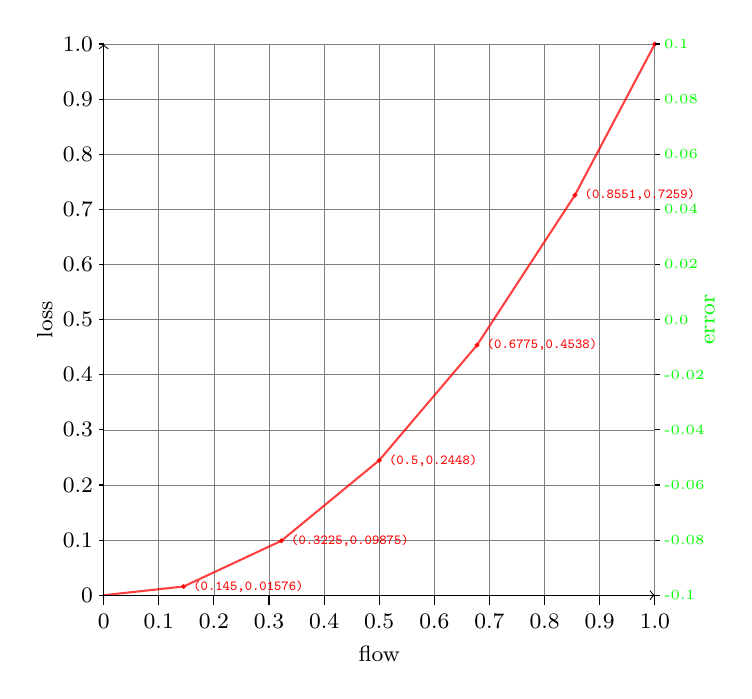
\begin{tikzpicture}[xscale=7.0,yscale=7.0]
\draw [help lines,step=0.1] (0,0) grid (1,1);
\draw[line width=0.5pt,color=black] plot file {default_6_XY.dat};
\coordinate (oneone) at (1,1);
\filldraw [red,draw opacity=0.75] (oneone) circle (0.1pt);
\coordinate (bk1) at (0,0);
\coordinate (bk2) at (0.14497,0.015762);
\coordinate (bk3) at (0.3225,0.098752);
\coordinate (bk4) at (0.50002,0.24477);
\coordinate (bk5) at (0.67754,0.45381);
\coordinate (bk6) at (0.85506,0.72587);
\coordinate (bk7) at (1,1);
\filldraw [red,draw opacity=0.75] (bk2) circle (0.1pt) node[right] {\tiny \texttt{(0.145,0.01576)}};
\filldraw [red,draw opacity=0.75] (bk3) circle (0.1pt) node[right] {\tiny \texttt{(0.3225,0.09875)}};
\filldraw [red,draw opacity=0.75] (bk4) circle (0.1pt) node[right] {\tiny \texttt{(0.5,0.2448)}};
\filldraw [red,draw opacity=0.75] (bk5) circle (0.1pt) node[right] {\tiny \texttt{(0.6775,0.4538)}};
\filldraw [red,draw opacity=0.75] (bk6) circle (0.1pt) node[right] {\tiny \texttt{(0.8551,0.7259)}};
\draw[line width=0.75pt,color=red,draw opacity=0.75] (bk1) -- (bk2); 
\draw[line width=0.75pt,color=red,draw opacity=0.75] (bk2) -- (bk3); 
\draw[line width=0.75pt,color=red,draw opacity=0.75] (bk3) -- (bk4); 
\draw[line width=0.75pt,color=red,draw opacity=0.75] (bk4) -- (bk5); 
\draw[line width=0.75pt,color=red,draw opacity=0.75] (bk5) -- (bk6); 
\draw[line width=0.75pt,color=red,draw opacity=0.75] (bk6) -- (bk7); 
\draw[->] (0,0) -- node[midway,yshift=-0.75cm] {\footnotesize flow} (1,0);
\draw[->] (0,0) -- node[rotate=90,midway,yshift=0.75cm] {\footnotesize loss} (0,1) ;
\foreach \x/\xtext in {0,0.1,0.2,0.3,0.4,0.5,0.6,0.7,0.8,0.9,1.0}
\draw (\x cm,0pt) -- (\x cm,-0.5pt) node[anchor=north] {\footnotesize \xtext};
\foreach \y/\ytext in {0,0.1,0.2,0.3,0.4,0.5,0.6,0.7,0.8,0.9,1.0}
\draw (0.0pt,\y cm) -- (-0.25pt,\y cm) node[anchor=east,xshift=0.5mm] {\footnotesize \ytext};
\draw[line width=0.5pt,color=green,draw opacity=0.75] plot file {default_6_err.dat};
\foreach \y/\ytext in {0/-0.1,0.1/-0.08,0.2/-0.06,0.3/-0.04,0.4/-0.02,0.5/0.0,0.6/0.02,0.7/0.04,0.8/0.06,0.9/0.08,1.0/0.1}
\draw (1cm,\y cm) -- (1.01cm,\y cm) node[anchor=west,xshift=-0.75mm] {\tiny \textcolor{green}{\ytext}};
\node[rotate=90] at (1.1,0.5) {\footnotesize \textcolor{green}{error}};
\end{tikzpicture}

\end{center}
}

\section{Weighted with average circuit and transformer usage during 2010} 

\frame{
 \frametitle{Loss segment approximation -- 2 segments}
\vspace{-10mm}
\begin{center}
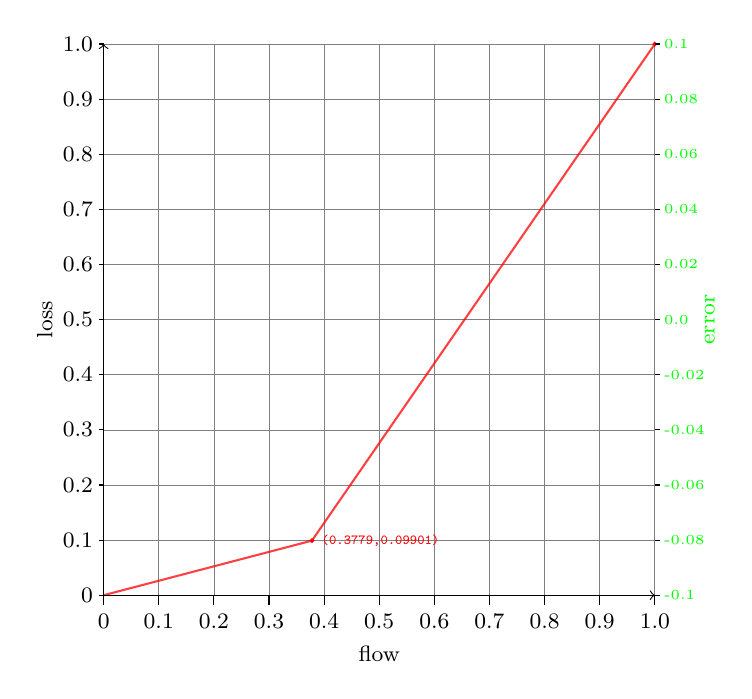
\begin{tikzpicture}[xscale=7.0,yscale=7.0]
\draw [help lines,step=0.1] (0,0) grid (1,1);
\filldraw[line width=0.5pt,color=blue!25!white,draw opacity=0.15,fill opacity = 0.5] plot file {tall_2_hg.dat};
\draw[line width=0.5pt,color=black] plot file {tall_2_XY.dat};
\coordinate (oneone) at (1,1);
\filldraw [red,draw opacity=0.75] (oneone) circle (0.1pt);
\coordinate (bk1) at (0,0);
\coordinate (bk2) at (0.37792,0.09901);
\coordinate (bk3) at (1,1);
\filldraw [red,draw opacity=0.75] (bk2) circle (0.1pt) node[right] {\tiny \texttt{(0.3779,0.09901)}};
\draw[line width=0.75pt,color=red,draw opacity=0.75] (bk1) -- (bk2); 
\draw[line width=0.75pt,color=red,draw opacity=0.75] (bk2) -- (bk3); 
\draw[->] (0,0) -- node[midway,yshift=-0.75cm] {\footnotesize flow} (1,0);
\draw[->] (0,0) -- node[rotate=90,midway,yshift=0.75cm] {\footnotesize loss} (0,1) ;
\foreach \x/\xtext in {0,0.1,0.2,0.3,0.4,0.5,0.6,0.7,0.8,0.9,1.0}
\draw (\x cm,0pt) -- (\x cm,-0.5pt) node[anchor=north] {\footnotesize \xtext};
\foreach \y/\ytext in {0,0.1,0.2,0.3,0.4,0.5,0.6,0.7,0.8,0.9,1.0}
\draw (0.0pt,\y cm) -- (-0.25pt,\y cm) node[anchor=east,xshift=0.5mm] {\footnotesize \ytext};
\draw[line width=0.5pt,color=green,draw opacity=0.75] plot file {tall_2_err.dat};
\foreach \y/\ytext in {0/-0.1,0.1/-0.08,0.2/-0.06,0.3/-0.04,0.4/-0.02,0.5/0.0,0.6/0.02,0.7/0.04,0.8/0.06,0.9/0.08,1.0/0.1}
\draw (1cm,\y cm) -- (1.01cm,\y cm) node[anchor=west,xshift=-0.75mm] {\tiny \textcolor{green}{\ytext}};
\node[rotate=90] at (1.1,0.5) {\footnotesize \textcolor{green}{error}};
\end{tikzpicture}

\end{center}
}

\frame{
 \frametitle{Loss segment approximation -- 3 segments}
\vspace{-10mm}
\begin{center}
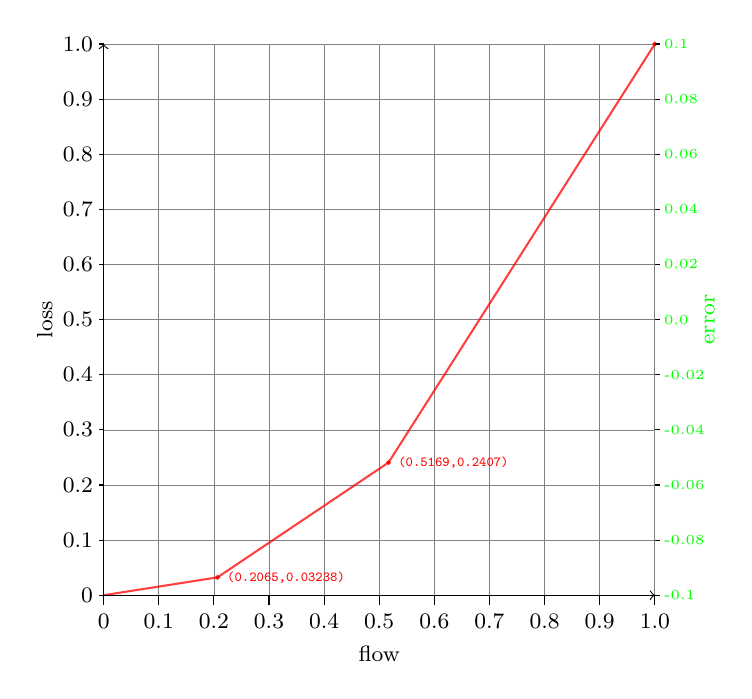
\begin{tikzpicture}[xscale=7.0,yscale=7.0]
\draw [help lines,step=0.1] (0,0) grid (1,1);
\filldraw[line width=0.5pt,color=blue!25!white,draw opacity=0.15,fill opacity = 0.5] plot file {tall_3_hg.dat};
\draw[line width=0.5pt,color=black] plot file {tall_3_XY.dat};
\coordinate (oneone) at (1,1);
\filldraw [red,draw opacity=0.75] (oneone) circle (0.1pt);
\coordinate (bk1) at (0,0);
\coordinate (bk2) at (0.20653,0.032379);
\coordinate (bk3) at (0.51691,0.24074);
\coordinate (bk4) at (1,1);
\filldraw [red,draw opacity=0.75] (bk2) circle (0.1pt) node[right] {\tiny \texttt{(0.2065,0.03238)}};
\filldraw [red,draw opacity=0.75] (bk3) circle (0.1pt) node[right] {\tiny \texttt{(0.5169,0.2407)}};
\draw[line width=0.75pt,color=red,draw opacity=0.75] (bk1) -- (bk2); 
\draw[line width=0.75pt,color=red,draw opacity=0.75] (bk2) -- (bk3); 
\draw[line width=0.75pt,color=red,draw opacity=0.75] (bk3) -- (bk4); 
\draw[->] (0,0) -- node[midway,yshift=-0.75cm] {\footnotesize flow} (1,0);
\draw[->] (0,0) -- node[rotate=90,midway,yshift=0.75cm] {\footnotesize loss} (0,1) ;
\foreach \x/\xtext in {0,0.1,0.2,0.3,0.4,0.5,0.6,0.7,0.8,0.9,1.0}
\draw (\x cm,0pt) -- (\x cm,-0.5pt) node[anchor=north] {\footnotesize \xtext};
\foreach \y/\ytext in {0,0.1,0.2,0.3,0.4,0.5,0.6,0.7,0.8,0.9,1.0}
\draw (0.0pt,\y cm) -- (-0.25pt,\y cm) node[anchor=east,xshift=0.5mm] {\footnotesize \ytext};
\draw[line width=0.5pt,color=green,draw opacity=0.75] plot file {tall_3_err.dat};
\foreach \y/\ytext in {0/-0.1,0.1/-0.08,0.2/-0.06,0.3/-0.04,0.4/-0.02,0.5/0.0,0.6/0.02,0.7/0.04,0.8/0.06,0.9/0.08,1.0/0.1}
\draw (1cm,\y cm) -- (1.01cm,\y cm) node[anchor=west,xshift=-0.75mm] {\tiny \textcolor{green}{\ytext}};
\node[rotate=90] at (1.1,0.5) {\footnotesize \textcolor{green}{error}};
\end{tikzpicture}

\end{center}
}

\frame{
 \frametitle{Loss segment approximation -- 4 segments}
\vspace{-10mm}
\begin{center}
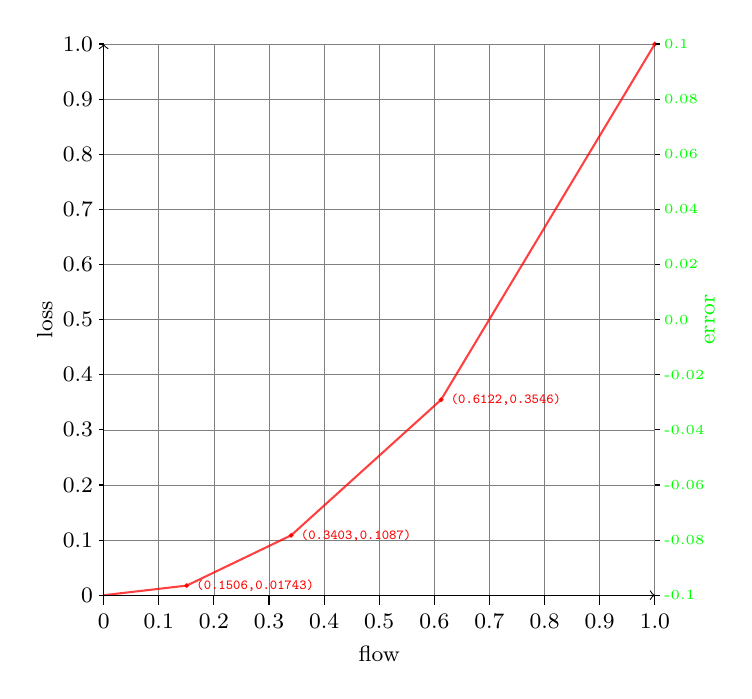
\begin{tikzpicture}[xscale=7.0,yscale=7.0]
\draw [help lines,step=0.1] (0,0) grid (1,1);
\filldraw[line width=0.5pt,color=blue!25!white,draw opacity=0.15,fill opacity = 0.5] plot file {tall_4_hg.dat};
\draw[line width=0.5pt,color=black] plot file {tall_4_XY.dat};
\coordinate (oneone) at (1,1);
\filldraw [red,draw opacity=0.75] (oneone) circle (0.1pt);
\coordinate (bk1) at (0,0);
\coordinate (bk2) at (0.15064,0.017431);
\coordinate (bk3) at (0.3403,0.10867);
\coordinate (bk4) at (0.6122,0.35461);
\coordinate (bk5) at (1,1);
\filldraw [red,draw opacity=0.75] (bk2) circle (0.1pt) node[right] {\tiny \texttt{(0.1506,0.01743)}};
\filldraw [red,draw opacity=0.75] (bk3) circle (0.1pt) node[right] {\tiny \texttt{(0.3403,0.1087)}};
\filldraw [red,draw opacity=0.75] (bk4) circle (0.1pt) node[right] {\tiny \texttt{(0.6122,0.3546)}};
\draw[line width=0.75pt,color=red,draw opacity=0.75] (bk1) -- (bk2); 
\draw[line width=0.75pt,color=red,draw opacity=0.75] (bk2) -- (bk3); 
\draw[line width=0.75pt,color=red,draw opacity=0.75] (bk3) -- (bk4); 
\draw[line width=0.75pt,color=red,draw opacity=0.75] (bk4) -- (bk5); 
\draw[->] (0,0) -- node[midway,yshift=-0.75cm] {\footnotesize flow} (1,0);
\draw[->] (0,0) -- node[rotate=90,midway,yshift=0.75cm] {\footnotesize loss} (0,1) ;
\foreach \x/\xtext in {0,0.1,0.2,0.3,0.4,0.5,0.6,0.7,0.8,0.9,1.0}
\draw (\x cm,0pt) -- (\x cm,-0.5pt) node[anchor=north] {\footnotesize \xtext};
\foreach \y/\ytext in {0,0.1,0.2,0.3,0.4,0.5,0.6,0.7,0.8,0.9,1.0}
\draw (0.0pt,\y cm) -- (-0.25pt,\y cm) node[anchor=east,xshift=0.5mm] {\footnotesize \ytext};
\draw[line width=0.5pt,color=green,draw opacity=0.75] plot file {tall_4_err.dat};
\foreach \y/\ytext in {0/-0.1,0.1/-0.08,0.2/-0.06,0.3/-0.04,0.4/-0.02,0.5/0.0,0.6/0.02,0.7/0.04,0.8/0.06,0.9/0.08,1.0/0.1}
\draw (1cm,\y cm) -- (1.01cm,\y cm) node[anchor=west,xshift=-0.75mm] {\tiny \textcolor{green}{\ytext}};
\node[rotate=90] at (1.1,0.5) {\footnotesize \textcolor{green}{error}};
\end{tikzpicture}

\end{center}
}

\frame{
 \frametitle{Loss segment approximation - 5 segments}
\vspace{-10mm}
\begin{center}
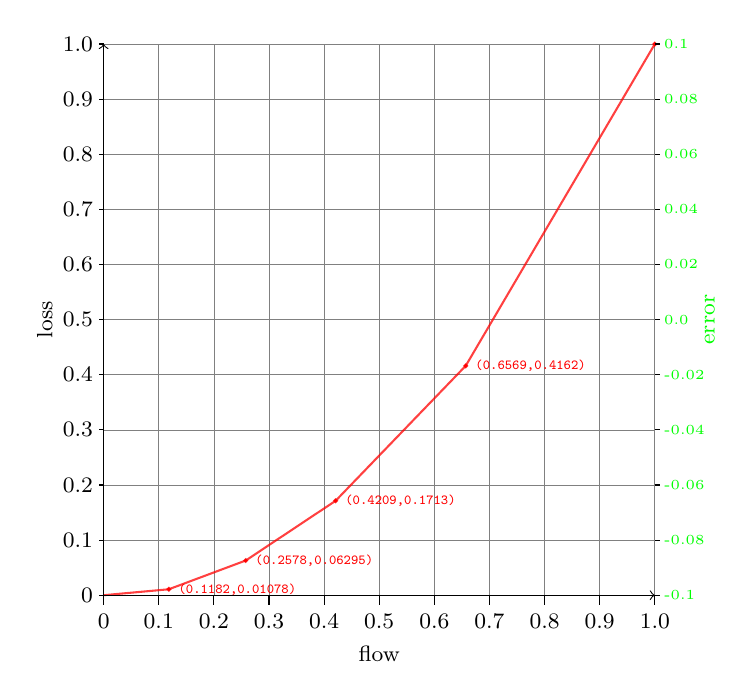
\begin{tikzpicture}[xscale=7.0,yscale=7.0]
\draw [help lines,step=0.1] (0,0) grid (1,1);
\filldraw[line width=0.5pt,color=blue!25!white,draw opacity=0.15,fill opacity = 0.5] plot file {tall_5_hg.dat};
\draw[line width=0.5pt,color=black] plot file {tall_5_XY.dat};
\coordinate (oneone) at (1,1);
\filldraw [red,draw opacity=0.75] (oneone) circle (0.1pt);
\coordinate (bk1) at (0,0);
\coordinate (bk2) at (0.11823,0.010782);
\coordinate (bk3) at (0.25778,0.06295);
\coordinate (bk4) at (0.42087,0.1713);
\coordinate (bk5) at (0.65692,0.41618);
\coordinate (bk6) at (1,1);
\filldraw [red,draw opacity=0.75] (bk2) circle (0.1pt) node[right] {\tiny \texttt{(0.1182,0.01078)}};
\filldraw [red,draw opacity=0.75] (bk3) circle (0.1pt) node[right] {\tiny \texttt{(0.2578,0.06295)}};
\filldraw [red,draw opacity=0.75] (bk4) circle (0.1pt) node[right] {\tiny \texttt{(0.4209,0.1713)}};
\filldraw [red,draw opacity=0.75] (bk5) circle (0.1pt) node[right] {\tiny \texttt{(0.6569,0.4162)}};
\draw[line width=0.75pt,color=red,draw opacity=0.75] (bk1) -- (bk2); 
\draw[line width=0.75pt,color=red,draw opacity=0.75] (bk2) -- (bk3); 
\draw[line width=0.75pt,color=red,draw opacity=0.75] (bk3) -- (bk4); 
\draw[line width=0.75pt,color=red,draw opacity=0.75] (bk4) -- (bk5); 
\draw[line width=0.75pt,color=red,draw opacity=0.75] (bk5) -- (bk6); 
\draw[->] (0,0) -- node[midway,yshift=-0.75cm] {\footnotesize flow} (1,0);
\draw[->] (0,0) -- node[rotate=90,midway,yshift=0.75cm] {\footnotesize loss} (0,1) ;
\foreach \x/\xtext in {0,0.1,0.2,0.3,0.4,0.5,0.6,0.7,0.8,0.9,1.0}
\draw (\x cm,0pt) -- (\x cm,-0.5pt) node[anchor=north] {\footnotesize \xtext};
\foreach \y/\ytext in {0,0.1,0.2,0.3,0.4,0.5,0.6,0.7,0.8,0.9,1.0}
\draw (0.0pt,\y cm) -- (-0.25pt,\y cm) node[anchor=east,xshift=0.5mm] {\footnotesize \ytext};
\draw[line width=0.5pt,color=green,draw opacity=0.75] plot file {tall_5_err.dat};
\foreach \y/\ytext in {0/-0.1,0.1/-0.08,0.2/-0.06,0.3/-0.04,0.4/-0.02,0.5/0.0,0.6/0.02,0.7/0.04,0.8/0.06,0.9/0.08,1.0/0.1}
\draw (1cm,\y cm) -- (1.01cm,\y cm) node[anchor=west,xshift=-0.75mm] {\tiny \textcolor{green}{\ytext}};
\node[rotate=90] at (1.1,0.5) {\footnotesize \textcolor{green}{error}};
\end{tikzpicture}

\end{center}
}

\frame{
 \frametitle{Loss segment approximation - 6 segments}
\vspace{-10mm}

\begin{center}
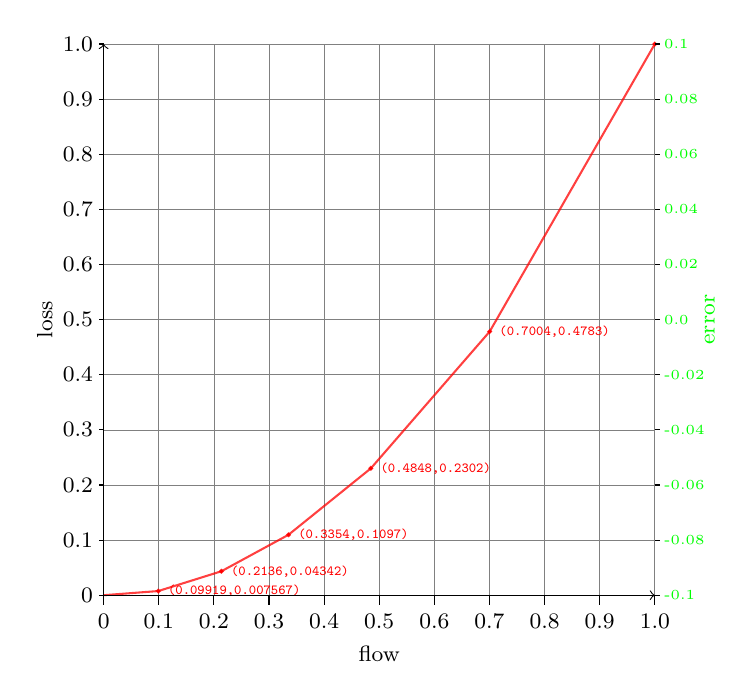
\begin{tikzpicture}[xscale=7.0,yscale=7.0]
\draw [help lines,step=0.1] (0,0) grid (1,1);
\filldraw[line width=0.5pt,color=blue!25!white,draw opacity=0.15,fill opacity = 0.5] plot file {tall_6_hg.dat};
\draw[line width=0.5pt,color=black] plot file {tall_6_XY.dat};
\coordinate (oneone) at (1,1);
\filldraw [red,draw opacity=0.75] (oneone) circle (0.1pt);
\coordinate (bk1) at (0,0);
\coordinate (bk2) at (0.099189,0.0075673);
\coordinate (bk3) at (0.2136,0.043423);
\coordinate (bk4) at (0.33542,0.10965);
\coordinate (bk5) at (0.48483,0.23016);
\coordinate (bk6) at (0.70036,0.47831);
\coordinate (bk7) at (1,1);
\filldraw [red,draw opacity=0.75] (bk2) circle (0.1pt) node[right] {\tiny \texttt{(0.09919,0.007567)}};
\filldraw [red,draw opacity=0.75] (bk3) circle (0.1pt) node[right] {\tiny \texttt{(0.2136,0.04342)}};
\filldraw [red,draw opacity=0.75] (bk4) circle (0.1pt) node[right] {\tiny \texttt{(0.3354,0.1097)}};
\filldraw [red,draw opacity=0.75] (bk5) circle (0.1pt) node[right] {\tiny \texttt{(0.4848,0.2302)}};
\filldraw [red,draw opacity=0.75] (bk6) circle (0.1pt) node[right] {\tiny \texttt{(0.7004,0.4783)}};
\draw[line width=0.75pt,color=red,draw opacity=0.75] (bk1) -- (bk2); 
\draw[line width=0.75pt,color=red,draw opacity=0.75] (bk2) -- (bk3); 
\draw[line width=0.75pt,color=red,draw opacity=0.75] (bk3) -- (bk4); 
\draw[line width=0.75pt,color=red,draw opacity=0.75] (bk4) -- (bk5); 
\draw[line width=0.75pt,color=red,draw opacity=0.75] (bk5) -- (bk6); 
\draw[line width=0.75pt,color=red,draw opacity=0.75] (bk6) -- (bk7); 
\draw[->] (0,0) -- node[midway,yshift=-0.75cm] {\footnotesize flow} (1,0);
\draw[->] (0,0) -- node[rotate=90,midway,yshift=0.75cm] {\footnotesize loss} (0,1) ;
\foreach \x/\xtext in {0,0.1,0.2,0.3,0.4,0.5,0.6,0.7,0.8,0.9,1.0}
\draw (\x cm,0pt) -- (\x cm,-0.5pt) node[anchor=north] {\footnotesize \xtext};
\foreach \y/\ytext in {0,0.1,0.2,0.3,0.4,0.5,0.6,0.7,0.8,0.9,1.0}
\draw (0.0pt,\y cm) -- (-0.25pt,\y cm) node[anchor=east,xshift=0.5mm] {\footnotesize \ytext};
\draw[line width=0.5pt,color=green,draw opacity=0.75] plot file {tall_6_err.dat};
\foreach \y/\ytext in {0/-0.1,0.1/-0.08,0.2/-0.06,0.3/-0.04,0.4/-0.02,0.5/0.0,0.6/0.02,0.7/0.04,0.8/0.06,0.9/0.08,1.0/0.1}
\draw (1cm,\y cm) -- (1.01cm,\y cm) node[anchor=west,xshift=-0.75mm] {\tiny \textcolor{green}{\ytext}};
\node[rotate=90] at (1.1,0.5) {\footnotesize \textcolor{green}{error}};
\end{tikzpicture}

\end{center}
}


\section{Transmission circuits loss segments (weighted with average circuit usage during 2010)} 

\frame{
 \frametitle{Loss segment approximation -- 2 segments}
\vspace{-10mm}
\begin{center}
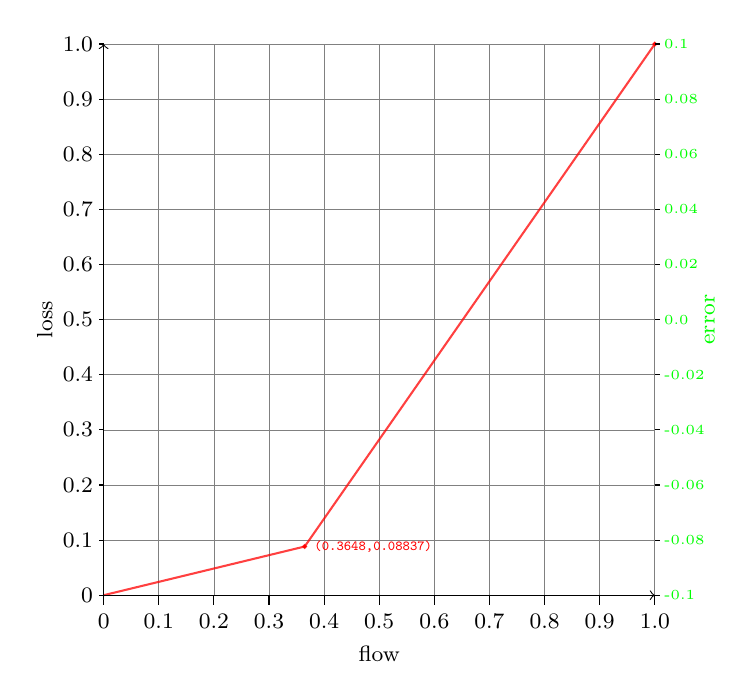
\begin{tikzpicture}[xscale=7.0,yscale=7.0]
\draw [help lines,step=0.1] (0,0) grid (1,1);
\filldraw[line width=0.5pt,color=blue!25!white,draw opacity=0.15,fill opacity = 0.5] plot file {tcuse_2_hg.dat};
\draw[line width=0.5pt,color=black] plot file {tcuse_2_XY.dat};
\coordinate (oneone) at (1,1);
\filldraw [red,draw opacity=0.75] (oneone) circle (0.1pt);
\coordinate (bk1) at (0,0);
\coordinate (bk2) at (0.36479,0.088371);
\coordinate (bk3) at (1,1);
\filldraw [red,draw opacity=0.75] (bk2) circle (0.1pt) node[right] {\tiny \texttt{(0.3648,0.08837)}};
\draw[line width=0.75pt,color=red,draw opacity=0.75] (bk1) -- (bk2); 
\draw[line width=0.75pt,color=red,draw opacity=0.75] (bk2) -- (bk3); 
\draw[->] (0,0) -- node[midway,yshift=-0.75cm] {\footnotesize flow} (1,0);
\draw[->] (0,0) -- node[rotate=90,midway,yshift=0.75cm] {\footnotesize loss} (0,1) ;
\foreach \x/\xtext in {0,0.1,0.2,0.3,0.4,0.5,0.6,0.7,0.8,0.9,1.0}
\draw (\x cm,0pt) -- (\x cm,-0.5pt) node[anchor=north] {\footnotesize \xtext};
\foreach \y/\ytext in {0,0.1,0.2,0.3,0.4,0.5,0.6,0.7,0.8,0.9,1.0}
\draw (0.0pt,\y cm) -- (-0.25pt,\y cm) node[anchor=east,xshift=0.5mm] {\footnotesize \ytext};
\draw[line width=0.5pt,color=green,draw opacity=0.75] plot file {tcuse_2_err.dat};
\foreach \y/\ytext in {0/-0.1,0.1/-0.08,0.2/-0.06,0.3/-0.04,0.4/-0.02,0.5/0.0,0.6/0.02,0.7/0.04,0.8/0.06,0.9/0.08,1.0/0.1}
\draw (1cm,\y cm) -- (1.01cm,\y cm) node[anchor=west,xshift=-0.75mm] {\tiny \textcolor{green}{\ytext}};
\node[rotate=90] at (1.1,0.5) {\footnotesize \textcolor{green}{error}};
\end{tikzpicture}

\end{center}
}

\frame{
 \frametitle{Loss segment approximation -- 3 segments}
\vspace{-10mm}
\begin{center}
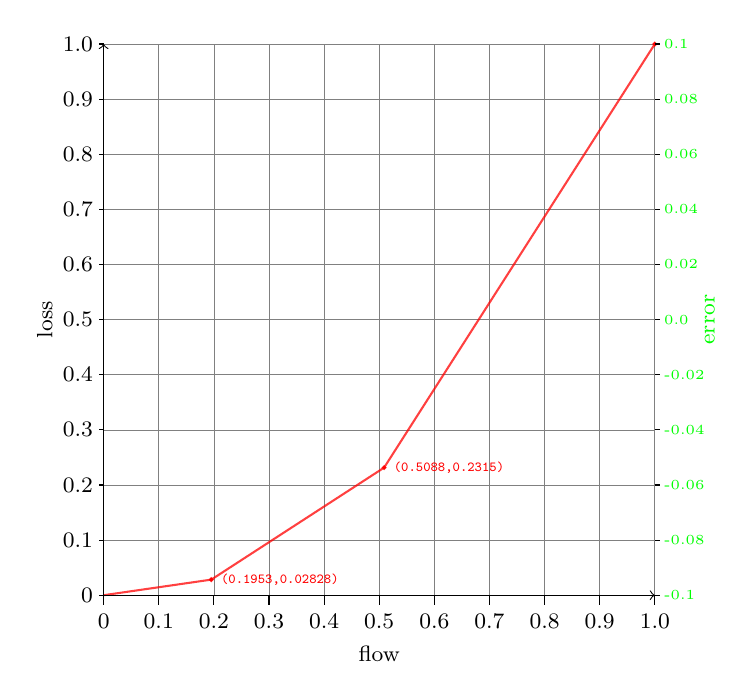
\begin{tikzpicture}[xscale=7.0,yscale=7.0]
\draw [help lines,step=0.1] (0,0) grid (1,1);
\filldraw[line width=0.5pt,color=blue!25!white,draw opacity=0.15,fill opacity = 0.5] plot file {tcuse_3_hg.dat};
\draw[line width=0.5pt,color=black] plot file {tcuse_3_XY.dat};
\coordinate (oneone) at (1,1);
\filldraw [red,draw opacity=0.75] (oneone) circle (0.1pt);
\coordinate (bk1) at (0,0);
\coordinate (bk2) at (0.1953,0.028279);
\coordinate (bk3) at (0.50885,0.23149);
\coordinate (bk4) at (1,1);
\filldraw [red,draw opacity=0.75] (bk2) circle (0.1pt) node[right] {\tiny \texttt{(0.1953,0.02828)}};
\filldraw [red,draw opacity=0.75] (bk3) circle (0.1pt) node[right] {\tiny \texttt{(0.5088,0.2315)}};
\draw[line width=0.75pt,color=red,draw opacity=0.75] (bk1) -- (bk2); 
\draw[line width=0.75pt,color=red,draw opacity=0.75] (bk2) -- (bk3); 
\draw[line width=0.75pt,color=red,draw opacity=0.75] (bk3) -- (bk4); 
\draw[->] (0,0) -- node[midway,yshift=-0.75cm] {\footnotesize flow} (1,0);
\draw[->] (0,0) -- node[rotate=90,midway,yshift=0.75cm] {\footnotesize loss} (0,1) ;
\foreach \x/\xtext in {0,0.1,0.2,0.3,0.4,0.5,0.6,0.7,0.8,0.9,1.0}
\draw (\x cm,0pt) -- (\x cm,-0.5pt) node[anchor=north] {\footnotesize \xtext};
\foreach \y/\ytext in {0,0.1,0.2,0.3,0.4,0.5,0.6,0.7,0.8,0.9,1.0}
\draw (0.0pt,\y cm) -- (-0.25pt,\y cm) node[anchor=east,xshift=0.5mm] {\footnotesize \ytext};
\draw[line width=0.5pt,color=green,draw opacity=0.75] plot file {tcuse_3_err.dat};
\foreach \y/\ytext in {0/-0.1,0.1/-0.08,0.2/-0.06,0.3/-0.04,0.4/-0.02,0.5/0.0,0.6/0.02,0.7/0.04,0.8/0.06,0.9/0.08,1.0/0.1}
\draw (1cm,\y cm) -- (1.01cm,\y cm) node[anchor=west,xshift=-0.75mm] {\tiny \textcolor{green}{\ytext}};
\node[rotate=90] at (1.1,0.5) {\footnotesize \textcolor{green}{error}};
\end{tikzpicture}

\end{center}
}

\frame{
 \frametitle{Loss segment approximation -- 4 segments}
\vspace{-10mm}
\begin{center}
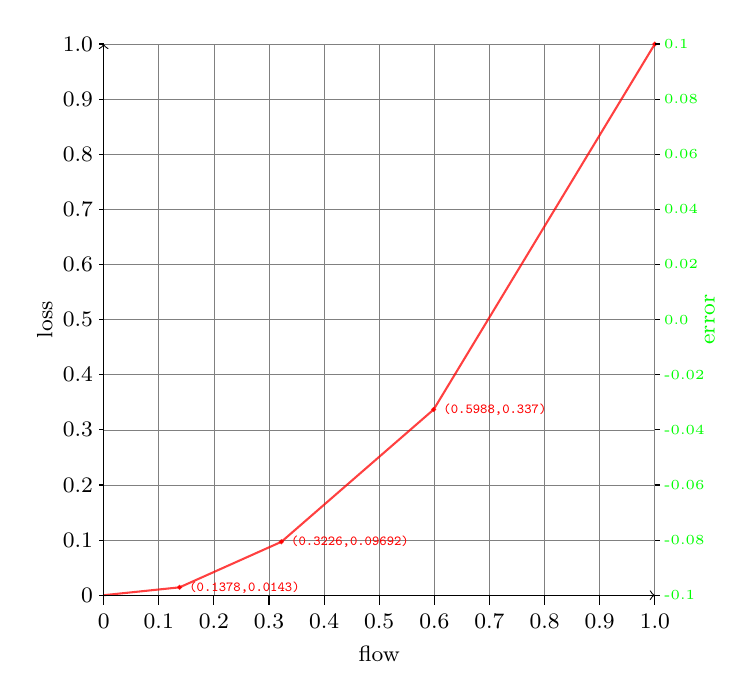
\begin{tikzpicture}[xscale=7.0,yscale=7.0]
\draw [help lines,step=0.1] (0,0) grid (1,1);
\filldraw[line width=0.5pt,color=blue!25!white,draw opacity=0.15,fill opacity = 0.5] plot file {tcuse_4_hg.dat};
\draw[line width=0.5pt,color=black] plot file {tcuse_4_XY.dat};
\coordinate (oneone) at (1,1);
\filldraw [red,draw opacity=0.75] (oneone) circle (0.1pt);
\coordinate (bk1) at (0,0);
\coordinate (bk2) at (0.13781,0.014302);
\coordinate (bk3) at (0.32256,0.096921);
\coordinate (bk4) at (0.59881,0.33698);
\coordinate (bk5) at (1,1);
\filldraw [red,draw opacity=0.75] (bk2) circle (0.1pt) node[right] {\tiny \texttt{(0.1378,0.0143)}};
\filldraw [red,draw opacity=0.75] (bk3) circle (0.1pt) node[right] {\tiny \texttt{(0.3226,0.09692)}};
\filldraw [red,draw opacity=0.75] (bk4) circle (0.1pt) node[right] {\tiny \texttt{(0.5988,0.337)}};
\draw[line width=0.75pt,color=red,draw opacity=0.75] (bk1) -- (bk2); 
\draw[line width=0.75pt,color=red,draw opacity=0.75] (bk2) -- (bk3); 
\draw[line width=0.75pt,color=red,draw opacity=0.75] (bk3) -- (bk4); 
\draw[line width=0.75pt,color=red,draw opacity=0.75] (bk4) -- (bk5); 
\draw[->] (0,0) -- node[midway,yshift=-0.75cm] {\footnotesize flow} (1,0);
\draw[->] (0,0) -- node[rotate=90,midway,yshift=0.75cm] {\footnotesize loss} (0,1) ;
\foreach \x/\xtext in {0,0.1,0.2,0.3,0.4,0.5,0.6,0.7,0.8,0.9,1.0}
\draw (\x cm,0pt) -- (\x cm,-0.5pt) node[anchor=north] {\footnotesize \xtext};
\foreach \y/\ytext in {0,0.1,0.2,0.3,0.4,0.5,0.6,0.7,0.8,0.9,1.0}
\draw (0.0pt,\y cm) -- (-0.25pt,\y cm) node[anchor=east,xshift=0.5mm] {\footnotesize \ytext};
\draw[line width=0.5pt,color=green,draw opacity=0.75] plot file {tcuse_4_err.dat};
\foreach \y/\ytext in {0/-0.1,0.1/-0.08,0.2/-0.06,0.3/-0.04,0.4/-0.02,0.5/0.0,0.6/0.02,0.7/0.04,0.8/0.06,0.9/0.08,1.0/0.1}
\draw (1cm,\y cm) -- (1.01cm,\y cm) node[anchor=west,xshift=-0.75mm] {\tiny \textcolor{green}{\ytext}};
\node[rotate=90] at (1.1,0.5) {\footnotesize \textcolor{green}{error}};
\end{tikzpicture}

\end{center}
}

\frame{
 \frametitle{Loss segment approximation - 5 segments}
\vspace{-10mm}
\begin{center}
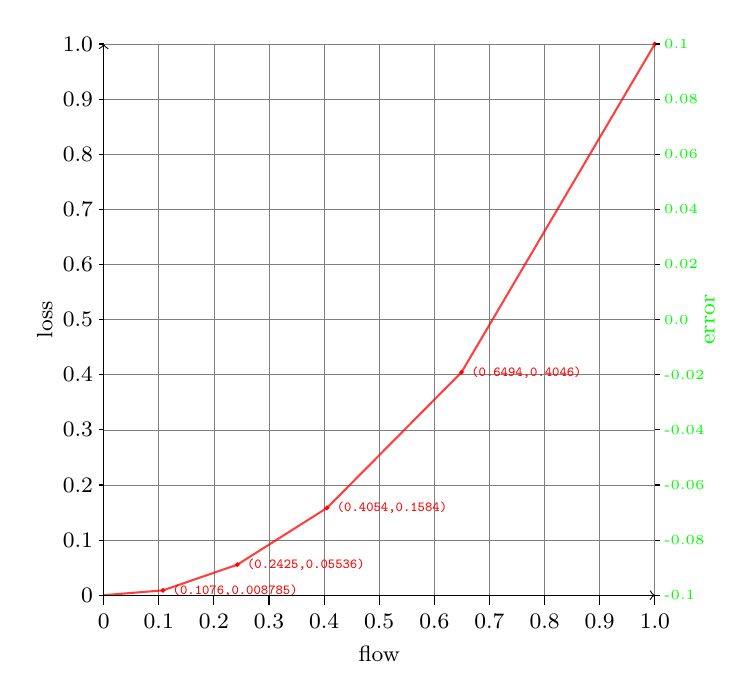
\begin{tikzpicture}[xscale=7.0,yscale=7.0]
\draw [help lines,step=0.1] (0,0) grid (1,1);
\filldraw[line width=0.5pt,color=blue!25!white,draw opacity=0.15,fill opacity = 0.5] plot file {tcuse_5_hg.dat};
\draw[line width=0.5pt,color=black] plot file {tcuse_5_XY.dat};
\coordinate (oneone) at (1,1);
\filldraw [red,draw opacity=0.75] (oneone) circle (0.1pt);
\coordinate (bk1) at (0,0);
\coordinate (bk2) at (0.10758,0.0087853);
\coordinate (bk3) at (0.24253,0.05536);
\coordinate (bk4) at (0.40538,0.15843);
\coordinate (bk5) at (0.6494,0.40463);
\coordinate (bk6) at (1,1);
\filldraw [red,draw opacity=0.75] (bk2) circle (0.1pt) node[right] {\tiny \texttt{(0.1076,0.008785)}};
\filldraw [red,draw opacity=0.75] (bk3) circle (0.1pt) node[right] {\tiny \texttt{(0.2425,0.05536)}};
\filldraw [red,draw opacity=0.75] (bk4) circle (0.1pt) node[right] {\tiny \texttt{(0.4054,0.1584)}};
\filldraw [red,draw opacity=0.75] (bk5) circle (0.1pt) node[right] {\tiny \texttt{(0.6494,0.4046)}};
\draw[line width=0.75pt,color=red,draw opacity=0.75] (bk1) -- (bk2); 
\draw[line width=0.75pt,color=red,draw opacity=0.75] (bk2) -- (bk3); 
\draw[line width=0.75pt,color=red,draw opacity=0.75] (bk3) -- (bk4); 
\draw[line width=0.75pt,color=red,draw opacity=0.75] (bk4) -- (bk5); 
\draw[line width=0.75pt,color=red,draw opacity=0.75] (bk5) -- (bk6); 
\draw[->] (0,0) -- node[midway,yshift=-0.75cm] {\footnotesize flow} (1,0);
\draw[->] (0,0) -- node[rotate=90,midway,yshift=0.75cm] {\footnotesize loss} (0,1) ;
\foreach \x/\xtext in {0,0.1,0.2,0.3,0.4,0.5,0.6,0.7,0.8,0.9,1.0}
\draw (\x cm,0pt) -- (\x cm,-0.5pt) node[anchor=north] {\footnotesize \xtext};
\foreach \y/\ytext in {0,0.1,0.2,0.3,0.4,0.5,0.6,0.7,0.8,0.9,1.0}
\draw (0.0pt,\y cm) -- (-0.25pt,\y cm) node[anchor=east,xshift=0.5mm] {\footnotesize \ytext};
\draw[line width=0.5pt,color=green,draw opacity=0.75] plot file {tcuse_5_err.dat};
\foreach \y/\ytext in {0/-0.1,0.1/-0.08,0.2/-0.06,0.3/-0.04,0.4/-0.02,0.5/0.0,0.6/0.02,0.7/0.04,0.8/0.06,0.9/0.08,1.0/0.1}
\draw (1cm,\y cm) -- (1.01cm,\y cm) node[anchor=west,xshift=-0.75mm] {\tiny \textcolor{green}{\ytext}};
\node[rotate=90] at (1.1,0.5) {\footnotesize \textcolor{green}{error}};
\end{tikzpicture}

\end{center}
}

\frame{
 \frametitle{Loss segment approximation - 6 segments}
\vspace{-10mm}

\begin{center}
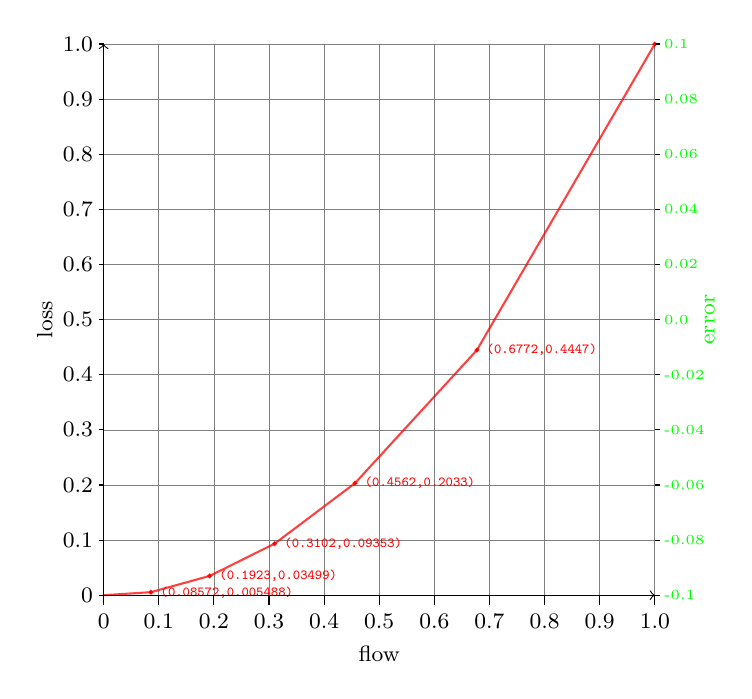
\begin{tikzpicture}[xscale=7.0,yscale=7.0]
\draw [help lines,step=0.1] (0,0) grid (1,1);
\filldraw[line width=0.5pt,color=blue!25!white,draw opacity=0.15,fill opacity = 0.5] plot file {tcuse_6_hg.dat};
\draw[line width=0.5pt,color=black] plot file {tcuse_6_XY.dat};
\coordinate (oneone) at (1,1);
\filldraw [red,draw opacity=0.75] (oneone) circle (0.1pt);
\coordinate (bk1) at (0,0);
\coordinate (bk2) at (0.085718,0.0054882);
\coordinate (bk3) at (0.19231,0.034989);
\coordinate (bk4) at (0.31023,0.093529);
\coordinate (bk5) at (0.45616,0.20334);
\coordinate (bk6) at (0.67722,0.44471);
\coordinate (bk7) at (1,1);
\filldraw [red,draw opacity=0.75] (bk2) circle (0.1pt) node[right] {\tiny \texttt{(0.08572,0.005488)}};
\filldraw [red,draw opacity=0.75] (bk3) circle (0.1pt) node[right] {\tiny \texttt{(0.1923,0.03499)}};
\filldraw [red,draw opacity=0.75] (bk4) circle (0.1pt) node[right] {\tiny \texttt{(0.3102,0.09353)}};
\filldraw [red,draw opacity=0.75] (bk5) circle (0.1pt) node[right] {\tiny \texttt{(0.4562,0.2033)}};
\filldraw [red,draw opacity=0.75] (bk6) circle (0.1pt) node[right] {\tiny \texttt{(0.6772,0.4447)}};
\draw[line width=0.75pt,color=red,draw opacity=0.75] (bk1) -- (bk2); 
\draw[line width=0.75pt,color=red,draw opacity=0.75] (bk2) -- (bk3); 
\draw[line width=0.75pt,color=red,draw opacity=0.75] (bk3) -- (bk4); 
\draw[line width=0.75pt,color=red,draw opacity=0.75] (bk4) -- (bk5); 
\draw[line width=0.75pt,color=red,draw opacity=0.75] (bk5) -- (bk6); 
\draw[line width=0.75pt,color=red,draw opacity=0.75] (bk6) -- (bk7); 
\draw[->] (0,0) -- node[midway,yshift=-0.75cm] {\footnotesize flow} (1,0);
\draw[->] (0,0) -- node[rotate=90,midway,yshift=0.75cm] {\footnotesize loss} (0,1) ;
\foreach \x/\xtext in {0,0.1,0.2,0.3,0.4,0.5,0.6,0.7,0.8,0.9,1.0}
\draw (\x cm,0pt) -- (\x cm,-0.5pt) node[anchor=north] {\footnotesize \xtext};
\foreach \y/\ytext in {0,0.1,0.2,0.3,0.4,0.5,0.6,0.7,0.8,0.9,1.0}
\draw (0.0pt,\y cm) -- (-0.25pt,\y cm) node[anchor=east,xshift=0.5mm] {\footnotesize \ytext};
\draw[line width=0.5pt,color=green,draw opacity=0.75] plot file {tcuse_6_err.dat};
\foreach \y/\ytext in {0/-0.1,0.1/-0.08,0.2/-0.06,0.3/-0.04,0.4/-0.02,0.5/0.0,0.6/0.02,0.7/0.04,0.8/0.06,0.9/0.08,1.0/0.1}
\draw (1cm,\y cm) -- (1.01cm,\y cm) node[anchor=west,xshift=-0.75mm] {\tiny \textcolor{green}{\ytext}};
\node[rotate=90] at (1.1,0.5) {\footnotesize \textcolor{green}{error}};
\end{tikzpicture}

\end{center}
}


\section{Transformer circuits loss segments (weighted with average circuit usage during 2010)} 

\frame{
 \frametitle{Loss segment approximation -- 2 segments}
\vspace{-10mm}
\begin{center}
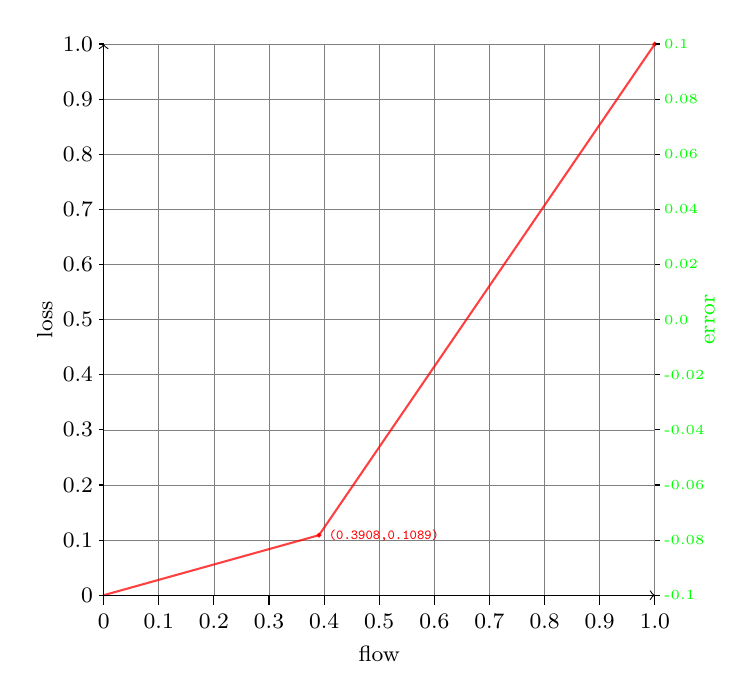
\begin{tikzpicture}[xscale=7.0,yscale=7.0]
\draw [help lines,step=0.1] (0,0) grid (1,1);
\filldraw[line width=0.5pt,color=blue!25!white,draw opacity=0.15,fill opacity = 0.5] plot file {txuse_2_hg.dat};
\draw[line width=0.5pt,color=black] plot file {txuse_2_XY.dat};
\coordinate (oneone) at (1,1);
\filldraw [red,draw opacity=0.75] (oneone) circle (0.1pt);
\coordinate (bk1) at (0,0);
\coordinate (bk2) at (0.39077,0.10894);
\coordinate (bk3) at (1,1);
\filldraw [red,draw opacity=0.75] (bk2) circle (0.1pt) node[right] {\tiny \texttt{(0.3908,0.1089)}};
\draw[line width=0.75pt,color=red,draw opacity=0.75] (bk1) -- (bk2); 
\draw[line width=0.75pt,color=red,draw opacity=0.75] (bk2) -- (bk3); 
\draw[->] (0,0) -- node[midway,yshift=-0.75cm] {\footnotesize flow} (1,0);
\draw[->] (0,0) -- node[rotate=90,midway,yshift=0.75cm] {\footnotesize loss} (0,1) ;
\foreach \x/\xtext in {0,0.1,0.2,0.3,0.4,0.5,0.6,0.7,0.8,0.9,1.0}
\draw (\x cm,0pt) -- (\x cm,-0.5pt) node[anchor=north] {\footnotesize \xtext};
\foreach \y/\ytext in {0,0.1,0.2,0.3,0.4,0.5,0.6,0.7,0.8,0.9,1.0}
\draw (0.0pt,\y cm) -- (-0.25pt,\y cm) node[anchor=east,xshift=0.5mm] {\footnotesize \ytext};
\draw[line width=0.5pt,color=green,draw opacity=0.75] plot file {txuse_2_err.dat};
\foreach \y/\ytext in {0/-0.1,0.1/-0.08,0.2/-0.06,0.3/-0.04,0.4/-0.02,0.5/0.0,0.6/0.02,0.7/0.04,0.8/0.06,0.9/0.08,1.0/0.1}
\draw (1cm,\y cm) -- (1.01cm,\y cm) node[anchor=west,xshift=-0.75mm] {\tiny \textcolor{green}{\ytext}};
\node[rotate=90] at (1.1,0.5) {\footnotesize \textcolor{green}{error}};
\end{tikzpicture}

\end{center}
}

\frame{
 \frametitle{Loss segment approximation -- 3 segments}
\vspace{-10mm}
\begin{center}
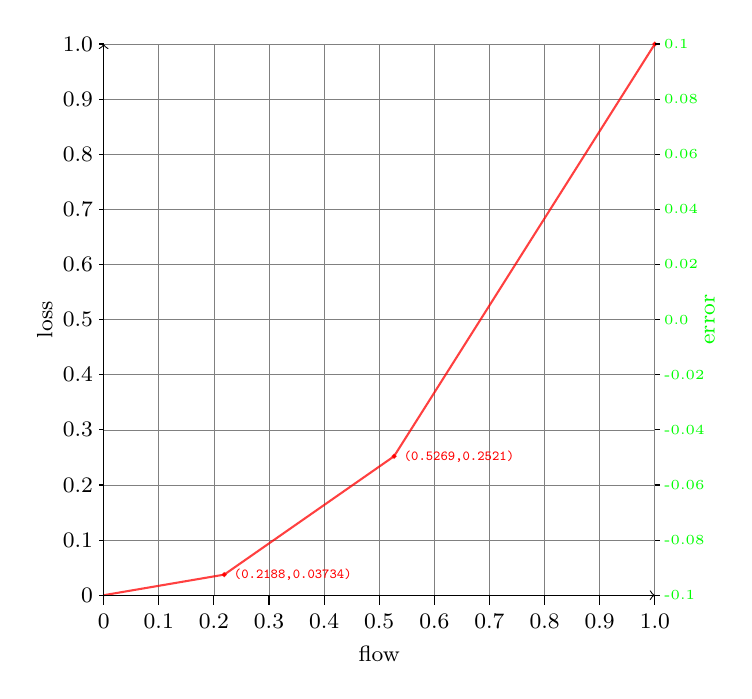
\begin{tikzpicture}[xscale=7.0,yscale=7.0]
\draw [help lines,step=0.1] (0,0) grid (1,1);
\filldraw[line width=0.5pt,color=blue!25!white,draw opacity=0.15,fill opacity = 0.5] plot file {txuse_3_hg.dat};
\draw[line width=0.5pt,color=black] plot file {txuse_3_XY.dat};
\coordinate (oneone) at (1,1);
\filldraw [red,draw opacity=0.75] (oneone) circle (0.1pt);
\coordinate (bk1) at (0,0);
\coordinate (bk2) at (0.21877,0.037337);
\coordinate (bk3) at (0.52691,0.25209);
\coordinate (bk4) at (1,1);
\filldraw [red,draw opacity=0.75] (bk2) circle (0.1pt) node[right] {\tiny \texttt{(0.2188,0.03734)}};
\filldraw [red,draw opacity=0.75] (bk3) circle (0.1pt) node[right] {\tiny \texttt{(0.5269,0.2521)}};
\draw[line width=0.75pt,color=red,draw opacity=0.75] (bk1) -- (bk2); 
\draw[line width=0.75pt,color=red,draw opacity=0.75] (bk2) -- (bk3); 
\draw[line width=0.75pt,color=red,draw opacity=0.75] (bk3) -- (bk4); 
\draw[->] (0,0) -- node[midway,yshift=-0.75cm] {\footnotesize flow} (1,0);
\draw[->] (0,0) -- node[rotate=90,midway,yshift=0.75cm] {\footnotesize loss} (0,1) ;
\foreach \x/\xtext in {0,0.1,0.2,0.3,0.4,0.5,0.6,0.7,0.8,0.9,1.0}
\draw (\x cm,0pt) -- (\x cm,-0.5pt) node[anchor=north] {\footnotesize \xtext};
\foreach \y/\ytext in {0,0.1,0.2,0.3,0.4,0.5,0.6,0.7,0.8,0.9,1.0}
\draw (0.0pt,\y cm) -- (-0.25pt,\y cm) node[anchor=east,xshift=0.5mm] {\footnotesize \ytext};
\draw[line width=0.5pt,color=green,draw opacity=0.75] plot file {txuse_3_err.dat};
\foreach \y/\ytext in {0/-0.1,0.1/-0.08,0.2/-0.06,0.3/-0.04,0.4/-0.02,0.5/0.0,0.6/0.02,0.7/0.04,0.8/0.06,0.9/0.08,1.0/0.1}
\draw (1cm,\y cm) -- (1.01cm,\y cm) node[anchor=west,xshift=-0.75mm] {\tiny \textcolor{green}{\ytext}};
\node[rotate=90] at (1.1,0.5) {\footnotesize \textcolor{green}{error}};
\end{tikzpicture}

\end{center}
}

\frame{
 \frametitle{Loss segment approximation -- 4 segments}
\vspace{-10mm}
\begin{center}
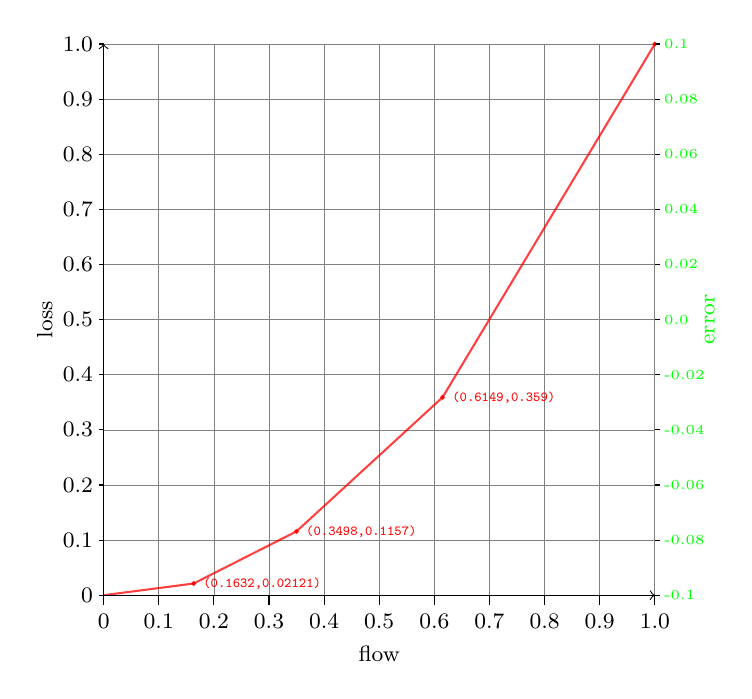
\begin{tikzpicture}[xscale=7.0,yscale=7.0]
\draw [help lines,step=0.1] (0,0) grid (1,1);
\filldraw[line width=0.5pt,color=blue!25!white,draw opacity=0.15,fill opacity = 0.5] plot file {txuse_4_hg.dat};
\draw[line width=0.5pt,color=black] plot file {txuse_4_XY.dat};
\coordinate (oneone) at (1,1);
\filldraw [red,draw opacity=0.75] (oneone) circle (0.1pt);
\coordinate (bk1) at (0,0);
\coordinate (bk2) at (0.16322,0.021208);
\coordinate (bk3) at (0.34979,0.11569);
\coordinate (bk4) at (0.6149,0.35903);
\coordinate (bk5) at (1,1);
\filldraw [red,draw opacity=0.75] (bk2) circle (0.1pt) node[right] {\tiny \texttt{(0.1632,0.02121)}};
\filldraw [red,draw opacity=0.75] (bk3) circle (0.1pt) node[right] {\tiny \texttt{(0.3498,0.1157)}};
\filldraw [red,draw opacity=0.75] (bk4) circle (0.1pt) node[right] {\tiny \texttt{(0.6149,0.359)}};
\draw[line width=0.75pt,color=red,draw opacity=0.75] (bk1) -- (bk2); 
\draw[line width=0.75pt,color=red,draw opacity=0.75] (bk2) -- (bk3); 
\draw[line width=0.75pt,color=red,draw opacity=0.75] (bk3) -- (bk4); 
\draw[line width=0.75pt,color=red,draw opacity=0.75] (bk4) -- (bk5); 
\draw[->] (0,0) -- node[midway,yshift=-0.75cm] {\footnotesize flow} (1,0);
\draw[->] (0,0) -- node[rotate=90,midway,yshift=0.75cm] {\footnotesize loss} (0,1) ;
\foreach \x/\xtext in {0,0.1,0.2,0.3,0.4,0.5,0.6,0.7,0.8,0.9,1.0}
\draw (\x cm,0pt) -- (\x cm,-0.5pt) node[anchor=north] {\footnotesize \xtext};
\foreach \y/\ytext in {0,0.1,0.2,0.3,0.4,0.5,0.6,0.7,0.8,0.9,1.0}
\draw (0.0pt,\y cm) -- (-0.25pt,\y cm) node[anchor=east,xshift=0.5mm] {\footnotesize \ytext};
\draw[line width=0.5pt,color=green,draw opacity=0.75] plot file {txuse_4_err.dat};
\foreach \y/\ytext in {0/-0.1,0.1/-0.08,0.2/-0.06,0.3/-0.04,0.4/-0.02,0.5/0.0,0.6/0.02,0.7/0.04,0.8/0.06,0.9/0.08,1.0/0.1}
\draw (1cm,\y cm) -- (1.01cm,\y cm) node[anchor=west,xshift=-0.75mm] {\tiny \textcolor{green}{\ytext}};
\node[rotate=90] at (1.1,0.5) {\footnotesize \textcolor{green}{error}};
\end{tikzpicture}

\end{center}
}

\frame{
 \frametitle{Loss segment approximation - 5 segments}
\vspace{-10mm}
\begin{center}
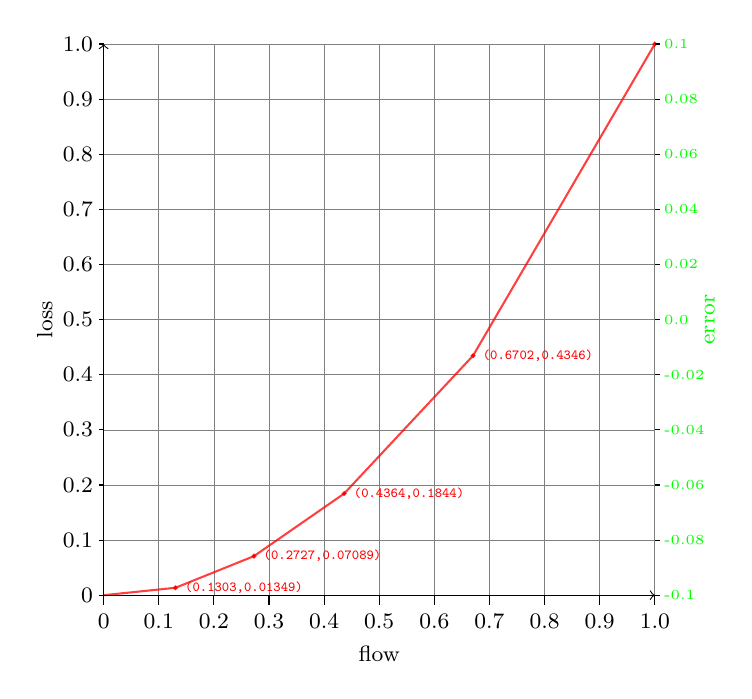
\begin{tikzpicture}[xscale=7.0,yscale=7.0]
\draw [help lines,step=0.1] (0,0) grid (1,1);
\filldraw[line width=0.5pt,color=blue!25!white,draw opacity=0.15,fill opacity = 0.5] plot file {txuse_5_hg.dat};
\draw[line width=0.5pt,color=black] plot file {txuse_5_XY.dat};
\coordinate (oneone) at (1,1);
\filldraw [red,draw opacity=0.75] (oneone) circle (0.1pt);
\coordinate (bk1) at (0,0);
\coordinate (bk2) at (0.13031,0.013493);
\coordinate (bk3) at (0.27269,0.070886);
\coordinate (bk4) at (0.43637,0.18438);
\coordinate (bk5) at (0.67024,0.43462);
\coordinate (bk6) at (1,1);
\filldraw [red,draw opacity=0.75] (bk2) circle (0.1pt) node[right] {\tiny \texttt{(0.1303,0.01349)}};
\filldraw [red,draw opacity=0.75] (bk3) circle (0.1pt) node[right] {\tiny \texttt{(0.2727,0.07089)}};
\filldraw [red,draw opacity=0.75] (bk4) circle (0.1pt) node[right] {\tiny \texttt{(0.4364,0.1844)}};
\filldraw [red,draw opacity=0.75] (bk5) circle (0.1pt) node[right] {\tiny \texttt{(0.6702,0.4346)}};
\draw[line width=0.75pt,color=red,draw opacity=0.75] (bk1) -- (bk2); 
\draw[line width=0.75pt,color=red,draw opacity=0.75] (bk2) -- (bk3); 
\draw[line width=0.75pt,color=red,draw opacity=0.75] (bk3) -- (bk4); 
\draw[line width=0.75pt,color=red,draw opacity=0.75] (bk4) -- (bk5); 
\draw[line width=0.75pt,color=red,draw opacity=0.75] (bk5) -- (bk6); 
\draw[->] (0,0) -- node[midway,yshift=-0.75cm] {\footnotesize flow} (1,0);
\draw[->] (0,0) -- node[rotate=90,midway,yshift=0.75cm] {\footnotesize loss} (0,1) ;
\foreach \x/\xtext in {0,0.1,0.2,0.3,0.4,0.5,0.6,0.7,0.8,0.9,1.0}
\draw (\x cm,0pt) -- (\x cm,-0.5pt) node[anchor=north] {\footnotesize \xtext};
\foreach \y/\ytext in {0,0.1,0.2,0.3,0.4,0.5,0.6,0.7,0.8,0.9,1.0}
\draw (0.0pt,\y cm) -- (-0.25pt,\y cm) node[anchor=east,xshift=0.5mm] {\footnotesize \ytext};
\draw[line width=0.5pt,color=green,draw opacity=0.75] plot file {txuse_5_err.dat};
\foreach \y/\ytext in {0/-0.1,0.1/-0.08,0.2/-0.06,0.3/-0.04,0.4/-0.02,0.5/0.0,0.6/0.02,0.7/0.04,0.8/0.06,0.9/0.08,1.0/0.1}
\draw (1cm,\y cm) -- (1.01cm,\y cm) node[anchor=west,xshift=-0.75mm] {\tiny \textcolor{green}{\ytext}};
\node[rotate=90] at (1.1,0.5) {\footnotesize \textcolor{green}{error}};
\end{tikzpicture}

\end{center}
}

\frame{
 \frametitle{Loss segment approximation - 6 segments}
\vspace{-10mm}

\begin{center}
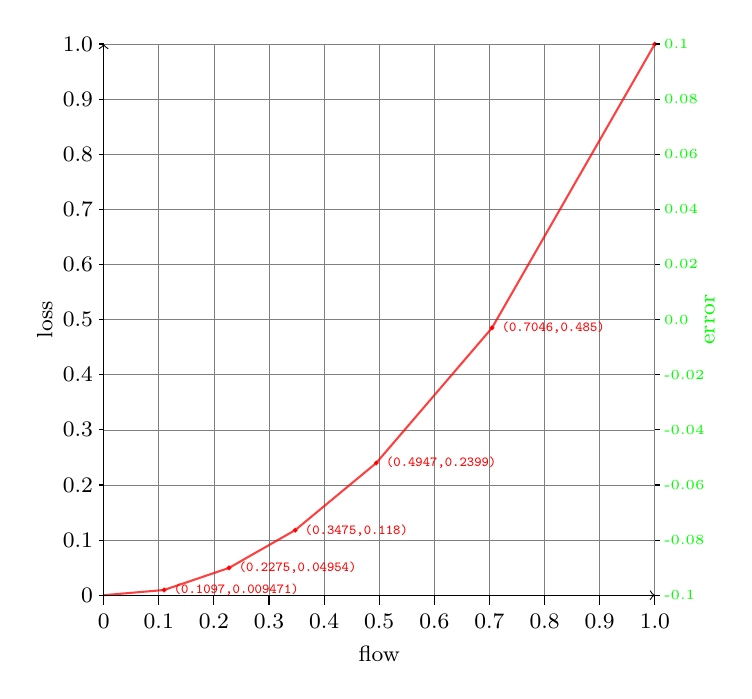
\begin{tikzpicture}[xscale=7.0,yscale=7.0]
\draw [help lines,step=0.1] (0,0) grid (1,1);
\filldraw[line width=0.5pt,color=blue!25!white,draw opacity=0.15,fill opacity = 0.5] plot file {txuse_6_hg.dat};
\draw[line width=0.5pt,color=black] plot file {txuse_6_XY.dat};
\coordinate (oneone) at (1,1);
\filldraw [red,draw opacity=0.75] (oneone) circle (0.1pt);
\coordinate (bk1) at (0,0);
\coordinate (bk2) at (0.10967,0.0094711);
\coordinate (bk3) at (0.22749,0.049541);
\coordinate (bk4) at (0.3475,0.11803);
\coordinate (bk5) at (0.49465,0.23992);
\coordinate (bk6) at (0.70464,0.485);
\coordinate (bk7) at (1,1);
\filldraw [red,draw opacity=0.75] (bk2) circle (0.1pt) node[right] {\tiny \texttt{(0.1097,0.009471)}};
\filldraw [red,draw opacity=0.75] (bk3) circle (0.1pt) node[right] {\tiny \texttt{(0.2275,0.04954)}};
\filldraw [red,draw opacity=0.75] (bk4) circle (0.1pt) node[right] {\tiny \texttt{(0.3475,0.118)}};
\filldraw [red,draw opacity=0.75] (bk5) circle (0.1pt) node[right] {\tiny \texttt{(0.4947,0.2399)}};
\filldraw [red,draw opacity=0.75] (bk6) circle (0.1pt) node[right] {\tiny \texttt{(0.7046,0.485)}};
\draw[line width=0.75pt,color=red,draw opacity=0.75] (bk1) -- (bk2); 
\draw[line width=0.75pt,color=red,draw opacity=0.75] (bk2) -- (bk3); 
\draw[line width=0.75pt,color=red,draw opacity=0.75] (bk3) -- (bk4); 
\draw[line width=0.75pt,color=red,draw opacity=0.75] (bk4) -- (bk5); 
\draw[line width=0.75pt,color=red,draw opacity=0.75] (bk5) -- (bk6); 
\draw[line width=0.75pt,color=red,draw opacity=0.75] (bk6) -- (bk7); 
\draw[->] (0,0) -- node[midway,yshift=-0.75cm] {\footnotesize flow} (1,0);
\draw[->] (0,0) -- node[rotate=90,midway,yshift=0.75cm] {\footnotesize loss} (0,1) ;
\foreach \x/\xtext in {0,0.1,0.2,0.3,0.4,0.5,0.6,0.7,0.8,0.9,1.0}
\draw (\x cm,0pt) -- (\x cm,-0.5pt) node[anchor=north] {\footnotesize \xtext};
\foreach \y/\ytext in {0,0.1,0.2,0.3,0.4,0.5,0.6,0.7,0.8,0.9,1.0}
\draw (0.0pt,\y cm) -- (-0.25pt,\y cm) node[anchor=east,xshift=0.5mm] {\footnotesize \ytext};
\draw[line width=0.5pt,color=green,draw opacity=0.75] plot file {txuse_6_err.dat};
\foreach \y/\ytext in {0/-0.1,0.1/-0.08,0.2/-0.06,0.3/-0.04,0.4/-0.02,0.5/0.0,0.6/0.02,0.7/0.04,0.8/0.06,0.9/0.08,1.0/0.1}
\draw (1cm,\y cm) -- (1.01cm,\y cm) node[anchor=west,xshift=-0.75mm] {\tiny \textcolor{green}{\ytext}};
\node[rotate=90] at (1.1,0.5) {\footnotesize \textcolor{green}{error}};
\end{tikzpicture}

\end{center}
}



\end{document}
    